\documentclass[12pt, a4paper]{report}
\usepackage{booktabs}
\usepackage[utf8]{inputenc}
\usepackage{amsmath}
\usepackage{amsfonts}
\usepackage{amssymb}
\usepackage{graphicx}
\usepackage[margin=2.5cm]{geometry}
\usepackage{hyperref}
\usepackage{enumitem} 
\usepackage[dvipsnames]{xcolor}   
\usepackage{times}
\usepackage{float}
\usepackage{mathtools}
\usepackage{multirow}
\usepackage{subcaption}
\usepackage{hyperref}
\usepackage{tikz}
\usetikzlibrary{shapes, arrows.meta, positioning, fit, backgrounds, shadows, calc}
\usepackage[backend=biber,style=ieee]{biblatex}
\addbibresource{ref.bib}

\hypersetup{
    colorlinks=true,
    linkcolor=black,
    filecolor=magenta,
    urlcolor=cyan,
    pdftitle={MR_project},
    pdfpagemode=FullScreen,
}

\newcommand{\bs}[1]{\boldsymbol{#1}}
\newcommand{\dbs}[1]{\dot{\boldsymbol{#1}}}
\newcommand{\ddbs}[1]{\ddot{\boldsymbol{#1}}}
\newcommand{\ps}[3]{{\prescript{#1}{}{#2}_{#3}}}

\begin{document}

\begin{titlepage}
    
    \centering
    
    \includegraphics[width=0.4\textwidth]{images/logo.png}\par\vspace{6cm}
    {\huge Motion Retargeting for Grasping Tasks \par}
    \vspace{0.3cm}
    {\Large Mapping synergies from humans to robotic hands with dissimilar kinematics \par}
    \vspace{1cm}
    
    {\large A.A. 2024 - 2025 \par}  

    \vspace{2cm}
    \textcolor{gray}{Based on the work of G. Gioioso, G. Salvietti, M. Malvezzi, and D. Prattichizzo (2013), IEEE Transactions on Robotics}\cite{gioioso2013mapping}
    
    \vspace{6cm}
    
    \begin{flushright}
        Matteo Zamponi \\
        Luca Colamarino \\
        Giuseppe D'Addario \\
        Federico Tranzocchi \\
        \textit{Sapienza University of Rome}
    \end{flushright}
    
\end{titlepage}

\tableofcontents

\chapter{Introduction}\label{ch:Intro}

Robotic hands are becoming increasingly common in research and industry. Modern robotic hands often have many degrees of freedom (DoF) to imitate the dexterity of the human hand, which has over 20 DoF. However, controlling these high-DoF robotic hands is a complex task: while the human brain controls the hand easily using coordinated patterns called \textit{synergies} \cite{santello1998postural}, explicitly controlling 15 or more motors of a robotic hand would be impractical.

This project addresses the problem of \textit{motion retargeting} from a human hand to a non-anthropomorphic robotic hand. The goal is to leverage human hand synergies to control a robotic hand with a different kinematic structure to that of the human hand. To do this, we use an object-based mapping approach called the \textit{virtual sphere} method \cite{gioioso2013mapping}, which focuses on the interaction between the hand and the object being manipulated.

\section{The correspondence problem}
A major challenge in teleoperation is the \textit{correspondence problem}. Human hands and robotic hands are rarely identical: they usually have different bone lengths, different types of joints, and a different number of fingers. Because of these differences, standard mapping techniques fail to accurately translate human motion.
\begin{itemize}
    \item \textit{Joint-to-joint mapping}: this method copies the angles of the human joints directly to the robot. This is often impossible because the robot might have fewer joints than the human, or the joints might rotate around different axes, leading to unnatural poses.
    \item \textit{Fingertip mapping}: this method forces the robot's fingertips to follow the position of the human fingertips. Although this ensures contact points are reached, it ignores the position of the palm and the rest of the fingers, causing the robot hand to collide with itself or reach impossible configurations.
\end{itemize}

To solve this, we adopt an approach proposed by Gioioso et al. \cite{gioioso2013mapping} that works in the \textit{object domain}. Instead of mapping the anatomy of the hand directly, we map the effect that the hand has on a virtual object (a sphere) held in the hand.

\section{Synergy-driven input}
To control the robotic hand, we first need a reliable reconstruction of the human hand pose. In this project, we use the Weart TouchDIVER G1 haptic glove in Figure \ref{fig:weart_glove}, which provides the closure of three fingers (thumb, index, middle) and the abduction of the thumb, plus other measurements that are not of interest for this work.
\begin{figure}[htbp]
    \centering
    \includegraphics[width=0.25\textwidth]{images/weart_glove} 
    \caption{The Weart TouchDIVER G1 haptic glove. Image source: \cite{weart_website}.}
    \label{fig:weart_glove}
\end{figure}

To reconstruct the full hand pose from this limited input, we rely on a reconstruction system developed in a previous work by Primiceri et al. \cite{primiceri2025motion}. Their system uses neural networks to estimate the full human hand pose from the sparse glove data, based on the theory of \textit{postural synergies} \cite{santello1998postural}. We take this reconstructed hand pose as the input for our motion retargeting system, focusing on the mathematical translation of this motion to the robotic hand.

\section{Objective}
Our main goal is to implement and validate a robust pipeline that allows a human operator to control robotic hands with different kinematics in real-time. Specifically, we present an algorithm that creates a virtual sphere inside the human hand and maps its deformation and movement to the robotic hand. Thanks to the mapping in the domain of the manipulated object, we create a generalized kinematic solver that can handle different robotic structures (e.g., from a 5-fingered hand to a 3-fingered one, or a 2-fingered gripper) without needing to redesign the mapping for each case. Finally, we evaluate the performance of our system by *TODO: add evaluation details*.

\section{Structure}
The rest of this report is structured as follows. In Chapter \ref{Ch:background} we review the relevant literature on hand synergies and motion retargeting techniques. In Chapter \ref{Ch:framework} we provide a mathematical formulation of the virtual sphere method and our implementation details. In Chapter \ref{Ch:setup} we describe the system architecture, including the hardware and software components used. In Chapter \ref{Ch:results} we present the results of our experiments and evaluate the performance of the retargeting system. Finally, in Chapter \ref{Ch:conclusion} we summarize our findings and discuss potential future work.
\chapter{Background}\label{Ch:background}

\section{Postural synergies}
% santello's theory

\section{Motion retargeting strategies}
% joint-to-joint mapping + limitations, fingertip/Cartesian mapping + limitations

\section{Object-based retargeting}
% theory behind virtual sphere method, advantages
\chapter{Framework}\label{Ch:framework}

\section{Reference points and sphere definition}

\section{Interaction matrix}

\section{Retargeting control law}

\section{Redundancy resolution}
\chapter{Experimental setup}\label{Ch:setup}

In this chapter, we describe the complete hardware and software architecture developed to validate the proposed retargeting framework. We will go through the data flow from the input device to the simulation environment, the software implementation of the control algorithms, and the specific robotic hand models used in the experiments.

\section{System overview}
The motion retargeting pipeline shown in Figure \ref{fig:system_overview} is designed as a modular system composed of three main blocks: the \textit{input layer} (haptic glove and reconstruction server), the \textit{retargeting layer} (unity simulation and retargeting logic), and the \textit{output layer} (robotic hand models).

\begin{figure}[h!]
    \centering
    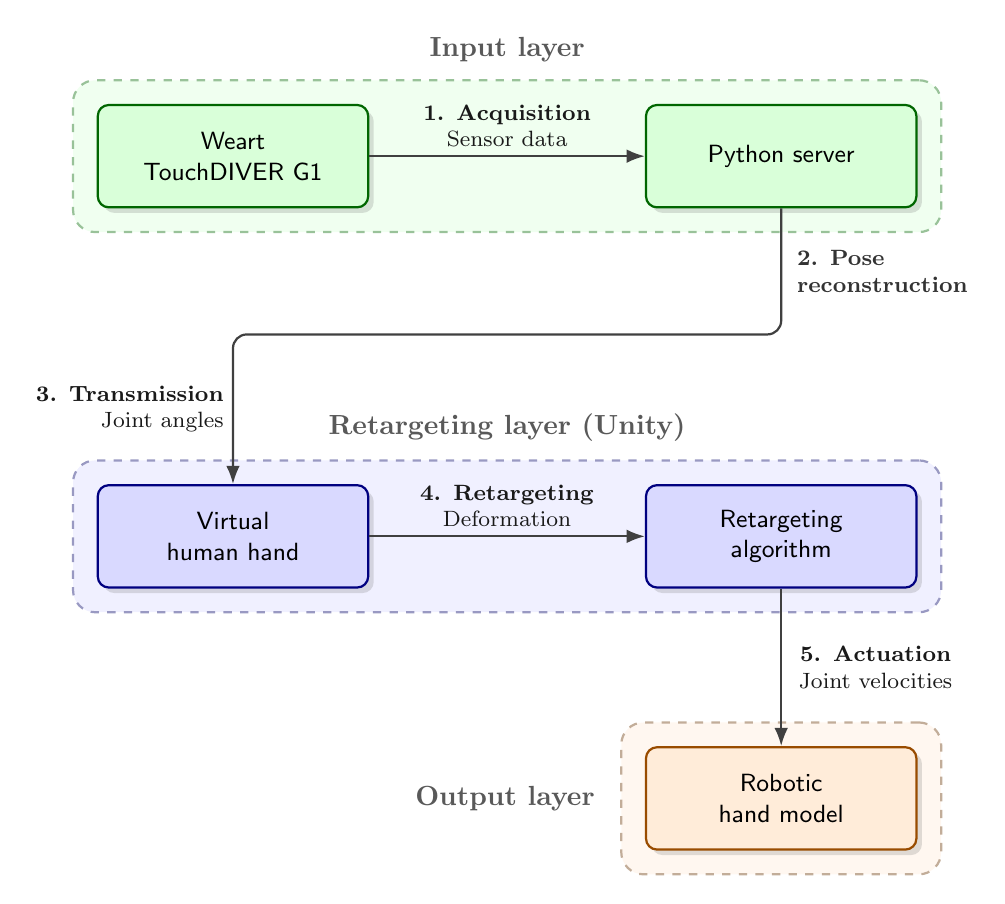
\begin{tikzpicture}[
        node distance=3.5cm and 3.5cm, 
        font=\small\sffamily,
        >=Latex,
        % styles
        baseBlock/.style={rectangle, thick, align=center, rounded corners=4pt, minimum height=1.3cm, text width=3.2cm, drop shadow={opacity=0.25, shadow xshift=2pt, shadow yshift=-2pt}},
        % component styles
        styleInput/.style={baseBlock, draw=green!40!black, fill=green!15},
        styleLogic/.style={baseBlock, draw=blue!50!black, fill=blue!15},
        styleOutput/.style={baseBlock, draw=orange!60!black, fill=orange!15},
        % container styles
        container/.style={dashed, thick, inner sep=0.3cm, rounded corners=8pt},
        cntInput/.style={container, draw=green!40!black!40, fill=green!6},
        cntLogic/.style={container, draw=blue!40!black!40, fill=blue!6},
        cntOutput/.style={container, draw=orange!40!black!40, fill=orange!6},
        % label styles
        layerLabel/.style={text=black!65, font=\bfseries, align=center},
        arrowLbl/.style={font=\footnotesize, align=center, text=black!90, inner sep=3pt},
        conn/.style={->, thick, draw=black!75, rounded corners=5pt}
    ]

    % nodes

    % row 1: input layer
    \node [styleInput] (glove) {Weart\\TouchDIVER G1};
    \node [styleInput, right=of glove] (server) {Python server};

    % row 2: retargeting layer
    \node [styleLogic, below=of glove] (vhand) {Virtual\\human hand};
    \node [styleLogic, right=of vhand] (algo) {Retargeting\\algorithm};

    % row 3: output layer
    \node [styleOutput, below=2.0cm of algo] (rhand) {Robotic\\hand model};

    % containers and labels
    \begin{scope}[on background layer]
        % block 1: input layer
        \node [cntInput, fit=(glove) (server)] (boxInput) {};
        \node [layerLabel, above=0.1cm of boxInput] {Input layer};
        
        % block 2: retargeting layer
        \node [cntLogic, fit=(vhand) (algo)] (boxLogic) {};
        \node [layerLabel, above=0.1cm of boxLogic] {Retargeting layer (Unity)};

        % block 3: output layer
        \node [cntOutput, fit=(rhand), minimum width=4cm] (boxOutput) {};
        \node [layerLabel, left=0.2cm of boxOutput, anchor=east] {Output layer};
    \end{scope}

    % connections

    % 1. Acquisition
    \draw [conn] (glove) -- node[arrowLbl, above] {\textbf{1. Acquisition}\\Sensor data} (server);

    % 2. Pose Reconstruction & 3. Transmission
    \draw [conn] (server.south) 
        -- ++(0,-1.6) coordinate(turn1) 
        node[midway, right, xshift=2pt, font=\footnotesize, text=black!80, align=left] {\textbf{2. Pose}\\ \textbf{reconstruction}}
        -- (turn1 -| vhand.north) coordinate(turn2) 
        -- (vhand.north)
        node[midway, left, arrowLbl, align=right] {\textbf{3. Transmission}\\Joint angles};

    % 4. Retargeting
    \draw [conn] (vhand) -- node[arrowLbl, above] {\textbf{4. Retargeting}\\Deformation} (algo);

    % 5. Actuation
    \draw [conn] (algo) -- node[arrowLbl, right, xshift=3pt] {\textbf{5. Actuation}\\Joint velocities} (rhand);

    \end{tikzpicture}
    \caption{System architecture overview showing the complete motion retargeting pipeline. The data flows from the haptic glove through the reconstruction server, into the Unity-based retargeting layer, and finally to the robotic hand model for actuation.}
    \label{fig:system_overview}
\end{figure}

The data flow consists of the following steps:
\begin{enumerate}
    \item \textit{Acquisition}: the user wears the Weart TouchDIVER G1 haptic glove, which captures sensor data (finger closure and abduction) that are sent to a Python server.
    \item \textit{Reconstruction}: the Python server processes the glove inputs using a neural network \cite{primiceri2025motion} to reconstruct the full pose of the virtual human hand in Unity.
    \item \textit{Transmission}: the reconstructed joint angles are sent to the Unity simulation environment in real-time.
    \item \textit{Retargeting}: inside Unity, the retargeting algorithm detailed in Chapter \ref{Ch:framework} computes the deformation of the virtual sphere and derives the corresponding joint velocities for the target robotic hand model.
    \item \textit{Actuation}: the resulting joint velocities are integrated to update the visual pose of the robotic hand in the simulation.
\end{enumerate}

\section{Human input layer}
The input interface is the Weart TouchDIVER G1, a wearable haptic device capable of tracking hand movements and rendering force, texture, and thermal cues. For the scope of this work, we focus on its motion tracking capabilities: it provides raw data about the closure of the thumb, index, and middle fingers, as well as the abduction of the thumb relative to the palm.

Since the glove does not track the ring and pinky fingers, nor the individual phalanx rotations (MCP, PIP, DIP) explicitly, the raw sensor data is insufficient for teleoperation. To address this limitation, we employ the reconstruction module developed by Primiceri et al. \cite{primiceri2025motion}: a Python script acts as a server listening for incoming data from the glove, and feeds this data into a pre-trained neural network which outputs a 62-dimensional vector containing the sine and cosine encodings of all 15 human hand joints; this vector is then converted back into Euler angles and sent to the Unity client.

\section{Software implementation}
The core logic of the project is implemented in C\# in the Unity engine. The implementation relies on the \texttt{MathNet.Numerics} library for efficient linear algebra computations, such as matrix multiplications and pseudoinverses.

\paragraph{Communication} A dedicated thread handles the TCP communication with the Python server to separate the network operations from the main Unity thread, so as to not interfere with the simulation's frame rate. The received human pose $\bs{q}_h$ is applied to a kinematic model of the human hand, which serves as the \textit{master} for the retargeting algorithm.

\paragraph{Kinematic solver} To guarantee the system is adaptable to different robots, we developed a generalized \texttt{Kinematics} library: unlike standard solutions that hardcode the Jacobian matrix for a specific robot, our implementation computes the robot Jacobian $\bs{J}_r$ dynamically. We define the robot structure in the Unity inspector by assigning a list of joint Transforms and their corresponding types (e.g., \texttt{HingeX}, \texttt{HingeY}, \texttt{HingeZ}, or \texttt{Ball}), allowing the software to handle any serial kinematic chain without code modification.

\paragraph{Virtual sphere} The \texttt{VirtualSphere} script implements the mathematical framework described in Chapter \ref{Ch:framework} for the deformation and retargeting logic. It takes as input an array of \texttt{Transform} objects representing the reference points, and at every update:
\begin{enumerate}
    \item it extracts the local positions of the reference points with respect to the palm;
    \item it computes the \textit{minimum enclosing ball} using Welzl's algorithm;
    \item it constructs the interaction matrix $\bs{A}$ from Eq. \refeq {eq:interaction_matrix} based on the sphere's current center and radius.
\end{enumerate}
This script is attached to both the human hand and the robotic hand, providing the necessary matrices $\bs{A}_h$ and $\bs{A}_r$ to the main controller.

\section{Robot models}
To evaluate the flexibility of the object-based retargeting approach \cite{gioioso2013mapping}, we selected robotic hands with significantly different kinematic structures to that of the human hand. In our experiments, we used two specific models: the \textit{Barrett Hand} and the \textit{Mia Hand}, whose kinematic descriptions (URDF models) were obtained from the embodiment framework by Fabisch et al. \cite{Fabisch2022}.

\subsection{Barrett Hand}
The \textit{Barrett Hand} (Figure \ref{fig:barrett_hand}) is a multi-fingered programmable grasper whose kinematic structure is deeply different from the human hand, making it an interesting candidate for testing the robustness of the virtual sphere retargeting method.

\begin{figure}[htbp]
    \centering
    \begin{subfigure}[b]{0.45\textwidth}
        \centering
        \includegraphics[width=0.55\textwidth]{images/barrett_hand1}
        \caption{Kinematic structure \cite{ros_barrett}}
        \label{fig:barrett_structure}
    \end{subfigure}
    \hfill
    \begin{subfigure}[b]{0.45\textwidth}
        \centering
        \includegraphics[width=0.95\textwidth]{images/barrett_hand2}
        \caption{Grasping an object \cite{barrett_website}}
        \label{fig:barrett_grasp}
    \end{subfigure}
    \caption{The Barrett Hand. (a) shows the hand in an open configuration, highlighting the three-finger design. (b) demonstrates the adaptability of the hand grasping an egg.}
    \label{fig:barrett_hand}
\end{figure}

\paragraph{Kinematics} It consists of three fingers: one finger is fixed, while the other two can rotate synchronously around the palm (\textit{spread motion}) up to $180^\circ$. This allows the hand to change its configuration dynamically, switching from a parallel grasp with the three fingers aligned, to an opposition grasp with the two rotating fingers opposing the fixed one.

\paragraph{Actuation} The hand has 8 axes of motion but is \textit{underactuated}, driven by only 4 motors: one controls the spread of the two movable fingers, and the other three control the flexion of each finger independently \cite{barrett_specs}. A proprietary "\textit{TorqueSwitch}" mechanism couples the proximal and distal links: the distal link remains stationary until the proximal link encounters resistance, at which point the distal link curls to enclose the object. However, we are interested in evaluating the retargeting performance based on kinematics alone; therefore, in our kinematic model of the Barrett Hand, we treat all 8 axes as independent degrees of freedom.

\subsection{Mia Hand}
The \textit{Mia Hand} (Figure \ref{fig:mia_hand}) by Prensilia is an anthropomorphic end-effector designed primarily for prosthetics and research applications. Unlike the Barrett Hand, the Mia Hand has a kinematic structure that resembles that of the human hand, although with less dexterity.

\begin{figure}[htbp]
    \centering
    \begin{subfigure}[b]{0.4\textwidth}
        \centering
        \includegraphics[width=0.8\textwidth]{images/mia_hand}
        \caption{Anthropomorphic structure \cite{prensilia_research}}
        \label{fig:mia_structure}
    \end{subfigure}
    \hspace{1cm}
    \begin{subfigure}[b]{0.4\textwidth}
        \centering
        \includegraphics[width=0.8\textwidth]{images/mia_hand_cylindrical_grip}
        \caption{Cylindrical grasp \cite{mia_grips}}
        \label{fig:mia_cylindrical}
    \end{subfigure}
    \caption{The Mia Hand. (a) shows the hand's resting posture, highlighting the mechanical design and soft pads. (b) shows the hand performing a cylindrical grasp, demonstrating finger coordination.}
    \label{fig:mia_hand}
\end{figure}

\paragraph{Kinematics} The Mia Hand's dimensions are similar to an average human hand (palm width 83 mm). It consists of five fingers and an opposable thumb, designed to perform various grasp types such as cylindrical, spherical, and lateral grasps \cite{mia_specs}.

\paragraph{Actuation} To keep a lightweight profile (approx. 540 g), the Mia Hand employs an underactuated mechanism driven by 3 motors actuating the flexion/extension of the fingers and the opposition of the thumb. Again, like for the Barrett Hand, in our simulation we treat the hand's kinematic chain as fully articulated, meaning we control the individual joints of the fingers independently. Consequently, the kinematic model has more degrees of freedom ($N \approx 15$) than the virtual sphere task ($N=7$), making the system \textit{kinematically redundant} with respect to it. We therefore employ the redundancy resolution strategy described in Chapter \ref{Ch:framework} to distribute the motion among the joints, keepeing them away from their mechanical limits while tracking the object deformation.
\chapter{Results}\label{Ch:results}

In this chapter, we present the experimental results obtained from the validation of the motion retargeting framework. The analysis is divided into two parts: a quantitative evaluation based on the metrics defined in Chapter \ref{Ch:setup}, and a qualitative assessment of the grasping capabilities on standard geometric objects.

The experiments were performed using the three robotic hands described in the previous chapter: the Barrett Hand, the Mia Hand, and the Shadow Dexterous Hand. For the quantitative analysis, we recorded data during a standardized grasping task where the user closes their hand (shrinking the virtual sphere, see Figure \ref{fig:sphere_grasp}) and translates it within the workspace. To isolate the performance of the retargeting algorithm from potential noise, these specific plots were generated using keyboard teleoperation to simulate a nominal closing motion. The qualitative validation, instead, uses the data recorded from the Weart Glove during natural human grasps.

\begin{figure}[htbp]
    \centering
    \begin{subfigure}[b]{0.3\textwidth}
        \centering
        \includegraphics[width=\textwidth]{images/VirtualSpheres/Barrett_Virtual_Sphere.png}
        \caption{Virtual sphere representation for the Barrett Hand.}
    \end{subfigure}
    \hfill
    \begin{subfigure}[b]{0.3\textwidth}
        \centering
        \includegraphics[width=\textwidth]{images/VirtualSpheres/Mia_Virtual_Sphere.png}
        \caption{Virtual sphere representation for the Mia Hand.}
    \end{subfigure}
    \hfill
    \begin{subfigure}[b]{0.3\textwidth}
        \centering
        \includegraphics[width=\textwidth]{images/VirtualSpheres/Shadow_Virtual_Sphere.png}
        \caption{Virtual sphere representation for the Shadow Dexterous Hand. On the left is the human hand, on the right the robot hand.}
    \end{subfigure}
    \caption{Virtual sphere representations for the robotic hands.}
    \label{fig:sphere_grasp}
\end{figure}

\section{Quantitative analysis}
We analyze the performance of the system in terms of geometric fidelity (radius and position tracking) and energetic fidelity (elastic energy estimation).

\subsection{Barrett Hand}
The Barrett Hand represents a significant test case due to its non-anthropomorphic structure and low number of actuated degrees of freedom (4 motors).

\begin{figure}[h!]
    \centering
    \includegraphics[width=0.55\textwidth]{images/Test/Barrett_GraspValidation.png}
    \caption{Performance metrics for the Barrett Hand.}
    \label{fig:results_barrett}
\end{figure}

\paragraph{Radius comparison} As shown in the top graph of Figure \ref{fig:results_barrett}, the retargeting algorithm succesfully maps the closing motion: the human hand (blue dashed line) starts the grasp at $t \approx 2.2$ s, reducing the virtual sphere radius from $\approx 0.17$ m to a steady-state value of $\approx 0.075$ m; the Barrett Hand (orange solid line) follows this reference closely. We can note how at first the robot radius slightly increases before starting to close, which may be due to the initial configuration.

We can also note how the robot achieves a smaller final radius ($\approx 0.06$ m) compared to the human hand, which is expected given the different kinematic structures: in fact, the Barrett Hand is capable of fully closing its fingers as we said in Chapter \ref{Ch:setup}, while the human hand cannot completely close around a sphere due to anatomical constraints.

\paragraph{Position variation} The middle graph illustrates the tracking of the hand position, represented by the center of the virtual sphere. The robot accurately follows the direction and profile of the human hand movement, with some differences in magnitude: the human hand translates by $\approx 0.11$ m, while the Barrett Hand reaches a displacement of $\approx 0.065$m. This is due to the physical parameters (stiffness, damping, force limit) we set for the imported URDF model of the Barrett Hand in the simulation environment in order to achieve stable grasps.

\paragraph{Elastic energy} The bottom graph shows the elastic potential energy stored in the grasp, which represents grasp intensity. We can identify two key observations: 
\begin{enumerate}
    \item there is a "lag" between the human input and the robot response (starting at $t \approx 2.3$ s for the human and $t \approx 2.4$ s for the robot). This is a consequence of the radius tracking performance discussed earlier, where the robot radius initially increases before closing;
    \item the steady-state energy of the robot stabilizes at a higher value ($\approx 0.37$ J) compared to the human reference ($\approx 0.25$ J), indicating a very firm grasp.
\end{enumerate}

\subsection{Mia Hand}
The Mia Hand shares the underactuated nature of the Barrett Hand but features an anthropomorphic design, as we discussed in Chapter \ref{Ch:setup}.

\begin{figure}[h!]
    \centering
    \includegraphics[width=0.55\textwidth]{images/Test/Mia_GraspValidation.png}
    \caption{Performance metrics for the Mia Hand.}
    \label{fig:results_mia}
\end{figure}

\paragraph{Radius comparison} From the top graph in Figure \ref{fig:results_mia} is clear that the Mia Hand tracks the human reference accurately during the closing motion, showing a similar trend to the Barrett Hand. However, in this case the radius does not exhibit an initial increase before starting to close.

\paragraph{Position variation} In the position tracking graph (middle), we observe that the Mia Hand adopts a more conservative approach compared to the Barrett Hand. While it follows the direction of the human hand movement, the overall displacement is smaller, with the Mia Hand translating by $\approx 0.04$ m compared to the human hand's $\approx 0.11$ m. This difference is again attributable to the tuning we performed on the physical parameters of the Mia Hand model in Unity.

\paragraph{Elastic energy} As for the energy plot (bottom), the main difference between the Mia Hand and the Barrett Hand is the absence of a lag in the robot response: the Mia Hand begins to store elastic energy at the same time as the human hand. The steady-state energy is again higher for the robot compared to the human reference, ensuring a firm grasp.

\subsection{Shadow Dexterous Hand}
The Shadow Dexterous Hand, being highly actuated and kinematically redundant for the grasping task, presents the closest approximation to the human hand among the three robotic hands considered.

\begin{figure}[h!]
    \centering
    \includegraphics[width=0.55\textwidth]{images/Test/Shadow_GraspValidation.png}
    \caption{Performance metrics for the Shadow Dexterous Hand.}
    \label{fig:results_shadow}
\end{figure}

\paragraph{Radius comparison} The radius tracking performance (top graph of Figure \ref{fig:results_shadow}) shows once again the initial increase in radius. Nonetheless, even in this case of a highly dexterous hand that is harder to control, the retargeting algorithm manages to follow the reference closing motion without significant issues or deviations.

\paragraph{Position variation} The motion of the virtual sphere of the Shadow Hand does not result in a substantial translation, with a displacement of only $\approx 0.02$ m. This conservative behavior is likely due to the high number of degrees of freedom and the complexity of coordinating them effectively during the grasping task.

\paragraph{Elastic energy} The energy profile (bottom) reports the same lag observed in the Barrett Hand case. Moreover, the main difference between this and the previous two hands lies in the steady-state energy level: this is the only hand that stabilizes at a lower energy ($\approx 0.11$ J) compared to the human reference. This could be already inferred from the radius plot, where the final robot radius is slightly larger than the human one, indicating a less intense grasp.

\section{Impact of redundancy resolution}
A key component of our control framework is the redundancy resolution strategy described in Chapter \ref{Ch:framework}, which exploits the null space of the robot Jacobian to optimize the internal configuration of the robot. This additional optimization did not show significant effects on the performance metrics analyzed in the previous section, as they only consider a single closing motion. Therefore, the primary task, that is tracking the virtual sphere so as to perform a stable grasp, can be achieved without leveraging redundancy, even in the case of the dexterous Shadow Hand. However, our experiments highlighted how redundancy resolution plays a crucial role when it comes to maintain a stable and natural behavior over time, when the user performs multiple grasps and releases in sequence.

\section{Qualitative validation}
The various grasping tasks with each robotic hand were performed on a ball, a cube, and a cylinder. These shapes were chosen for their simplicity and their ability to represent common grasping scenarios. In the following we show representative images of each robotic hand successfully grasping the objects using the motion retargeting framework.

\subsection{Barrett Hand}
The Barrett Hand demonstrated robust performance across all three test objects. In Figure \ref{fig:grasp_barrett} we can see how it effectively conforms to the shape of each object, achieving secure grasps: these resulted from an initial configuration where the three fingers were open in a claw-like posture.

\begin{figure}[htbp]
    \centering
    \begin{subfigure}[b]{0.3\textwidth}
        \centering
        \includegraphics[width=\textwidth]{images/Grasp/Barrett/Barrett_Grasp_Ball.png}
        \caption{Barrett Hand grasping a ball.}
    \end{subfigure}
    \hfill
    \begin{subfigure}[b]{0.3\textwidth}
        \centering
        \includegraphics[width=\textwidth]{images/Grasp/Barrett/Barrett_Grasp_Cube.png}
        \caption{Barrett Hand grasping a cube.}
    \end{subfigure}
    \hfill
    \begin{subfigure}[b]{0.3\textwidth}
        \centering
        \includegraphics[width=\textwidth]{images/Grasp/Barrett/Barrett_Grasp_Cylinder.png}
        \caption{Barrett Hand grasping a cylinder.}
    \end{subfigure}
    \caption{Barrett Hand grasping standard geometric objects.}
    \label{fig:grasp_barrett}
\end{figure}

\subsection{Mia Hand}
Figure \ref{fig:grasp_mia} shows the Mia Hand succesfully grasping the three objects from an initial open configuration. The anthropomorphic design and the underactuation of this hand allowed for a very simple yet effective grasping strategy, where the fingers naturally adapt to the shape of the objects upon collision.

\begin{figure}[htbp]
    \centering
    \begin{subfigure}[b]{0.3\textwidth}
        \centering
        \includegraphics[width=\textwidth]{images/Grasp/Mia/Mia_Grasp_Ball.png}
        \caption{Mia Hand grasping a ball.}
    \end{subfigure}
    \hfill
    \begin{subfigure}[b]{0.3\textwidth}
        \centering
        \includegraphics[width=\textwidth]{images/Grasp/Mia/Mia_Grasp_Cube.png}
        \caption{Mia Hand grasping a cube.}
    \end{subfigure}
    \hfill
    \begin{subfigure}[b]{0.3\textwidth}
        \centering
        \includegraphics[width=\textwidth]{images/Grasp/Mia/Mia_Grasp_Cylinder.png}
        \caption{Mia Hand grasping a cylinder.}
    \end{subfigure}
    \caption{Mia Hand grasping standard geometric objects.}
    \label{fig:grasp_mia}
\end{figure}

\subsection{Shadow Hand}
Finally, the Shadow Dexterous Hand showed some different behavior compared to the previous two robotic hands. Due to its high dexterity, it was harder for it to adapt to the simple closing motion of the human hand, resulting in some strange finger configurations during the grasps, as shown in Figure \ref{fig:grasp_shadow}.

\begin{figure}[htbp]
    \centering
    \begin{subfigure}[b]{0.3\textwidth}
        \centering
        \includegraphics[width=\textwidth]{images/Grasp/Shadow/Shadow_Grasp_Ball.png}
        \caption{Shadow Hand grasping a ball.}
    \end{subfigure}
    \hfill
    \begin{subfigure}[b]{0.3\textwidth}
        \centering
        \includegraphics[width=\textwidth]{images/Grasp/Shadow/Shadow_Grasp_Cube.png}
        \caption{Shadow Hand grasping a cube.}
    \end{subfigure}
    \hfill
    \begin{subfigure}[b]{0.3\textwidth}
        \centering
        \includegraphics[width=\textwidth]{images/Grasp/Shadow/Shadow_Grasp_Cylinder.png}
        \caption{Shadow Hand grasping a cylinder.}
    \end{subfigure}
    \caption{Shadow Hand grasping standard geometric objects.}
    \label{fig:grasp_shadow}
\end{figure}
\chapter{Conclusion}\label{Ch:conclusion}

In this work, we developed a system to control robotic hands using the motion of a human hand. We used a method called the \textit{virtual sphere}, which simplifies the problem by looking at how the hand interacts with an object rather than mapping the joints directly. We tested this system in a simulation with three different robotic hands: the Barrett Hand, the Mia Hand, and the Shadow Dexterous Hand.

\section{Summary}
Our experiments showed that the virtual sphere method is effective for controlling robotic hands with very different kinematic structures. Here is a summary of our main findings:
\begin{itemize}
    \item The system succesfully mapped the opening and closing of the human hand to all three robots, which managed to track the human radius changes well.
    \item All robots followed the direction of the human hand correctly, demonstrating the ability of the method to adapt to different initial configurations, which still affect the final grasping posture.
    \item The settings of the physical parameters of each robot, such as stiffness and damping, played a crucial role in the quality of the retargeted motion as well as the grasping success.
    \item The secondary objective of keeping the robot joints in their mid-range values did not have a significant impact on the single grasping tasks performed in this work. However, it showed a stabilizing effect on the robot posture in long sequences of motion, preventing extreme and unnatural joint configurations.
    \item All hands could grasp standard objects succesfully, proving that the method works for different shapes.
\end{itemize}

\section{Future work}
There are several ways to improve and extend this work in the future:
\begin{enumerate}
    \item So far, we have only tested the system in the Unity simulator. The next step is to connect real robotic hands to the system to see how friction, sensor noise, and communication delays affect performance in the real world.
    \item The Weart TouchDIVER glove can produce forces and vibrations. Currently, communication goes only one way (from glove to Unity). We could send collision data from Unity back to the glove so the user can feel the object being grasped.
    \item We used a sphere to represent the virtual object. Using different shapes, like an ellipsoid, might help grasp long or thin objects more accurately.
\end{enumerate}

\printbibliography

\end{document}